\documentclass[ucs,9pt,pagenumbersfull]{beamer}

\usetheme{gray}

%% To create high resolution - for print outs
%\usepackage{pgfpages}
%\pgfpagesuselayout{resize to}[a4paper,border shrink=5mm,landscape]
%\mode<handout>{\setbeamercolor{background canvas}{bg=black!5}}

\def\vRad{2pt} % Radius of vertices in TikZ images

\setbeameroption{hide notes}

\logosmall{logos/fu_small_logo}
\logobig{logos/fu_big_logo}
\logoaux{logos/cglLogo}
\logoauxx[1.cm]{logos/bms-logo-with-text}
\titleimage[2.92cm]{Figures/Title_picture}

\title[Contact Surfaces Parameterization] % (optional, use only with long paper titles)
{On the Parameterization and the \mbox{Geometry} of the \mbox{Configuration} Space of a Single \mbox{Planar} Robot}
% Optional subtitle
%\subtitle{Optional subtitle}

\author[Atariah,~Rote] % (optional, use only with lots of authors)
{Dror Atariah \and Günter Rote}
% - Give the names in the same order as the appear in the paper.

\institute[FU Berlin] % (optional, but mostly needed)
{Freie Universität Berlin}

\date[WSCG'13] % (optional, should be abbreviation of conference name)
{June 27\textsuperscript{th} 2013}
% - Either use conference name or its abbreviation.
% - Not really informative to the audience, more for people (including
%   yourself) who are reading the slides online

% Delete this, if you do not want the table of contents to pop up at
% the beginning of each subsection:
\AtBeginSection[]
{
  \begin{frame}<beamer>{Outline}
    \tableofcontents[currentsection]
  \end{frame}
}
\AtBeginSubsection[]
{
  \begin{frame}<beamer>{Outline}
    \tableofcontents[currentsubsection]
  \end{frame}
}

\begin{document}

\begin{frame}[plain]
  \titlepage
\end{frame}

\begin{frame}{Outline}
  \tableofcontents
  % You might wish to add the option [pausesections]
\end{frame}

\section{Introduction}

\begin{frame}
  \frametitle{Setting}
  \begin{columns}[c]
    \begin{column}{0.4\textwidth}
      \begin{minipage}[c][\textheight]{1.0\columnwidth}
          \onslide<1-2>{%
            A planar polygonal (convex) robot
            \(\mathcal{A}\) moving amid polygonal (convex) obstacles
            \(\{ \mathcal{O}_j \}_{j\in J}\).

            \begin{block}{Free\dots}
              Can be either in a \emph{free configuration}
              \(\mathcal{C}_{free}\).
            \end{block}%
          }%
          \onslide<2>{%
            \begin{block}{Forbidden\dots}
              \emph{Or,} forbidden one \(\mathcal{C}_{forb} =
              \mathcal{C} \setminus \mathcal{C}_{free} \).
            \end{block}
          }%
      \end{minipage}
    \end{column}
    \begin{column}{0.55\textwidth}
      \begin{minipage}[c][\textheight]{1.0\columnwidth}
        \centering
        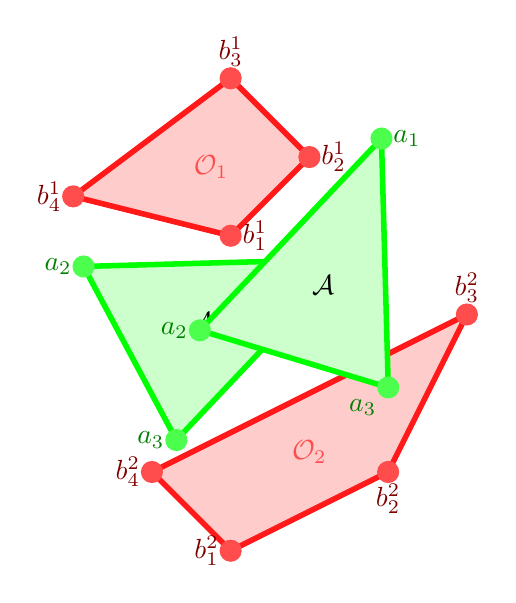
\begin{tikzpicture}[%
  obstacle/.style={line join=round,red!90,fill=red!20,line width=\vRad},
  obstacle vertices/.style={red!70},
  obstacle vertices label/.style={red!50!black},
  robot/.style={line join=round,green,fill=green!20,line width=\vRad},
  robot vertices/.style={green!70},
  robot vertices label/.style={green!50!black}
  ]

  \coordinate (b11) at (3,4);
  \coordinate (b12) at (4,5);
  \coordinate (b13) at (3,6);
  \coordinate (b14) at (1,4.5);

  \draw[obstacle] %
  (b11)node[obstacle vertices label,right]{$b_1^1$} --
  (b12)node[obstacle vertices label,right]{$b_2^1$} --
  (b13)node[obstacle vertices label,above]{$b_3^1$} --
  (b14)node[obstacle vertices label,left]{$b_4^1$} -- cycle;
  \foreach \i in {1,2,3,4}
  \fill[obstacle vertices] (b1\i) circle (2*\vRad);
  \node[obstacle vertices] at (barycentric cs:b11=0.25,b12=0.25,b13=0.25,b14=0.25) {$\mathcal{O}_1$};

  \coordinate (b21) at (3,0);
  \coordinate (b22) at (5,1);
  \coordinate (b23) at (6,3);
  \coordinate (b24) at (2,1);

  \draw[obstacle] %
  (b21)node[obstacle vertices label,left]{$b_1^2$} --
  (b22)node[obstacle vertices label,below]{$b_2^2$} --
  (b23)node[obstacle vertices label,above]{$b_3^2$} --
  (b24)node[obstacle vertices label,left]{$b_4^2$} -- cycle;
  \foreach \i in {1,2,3,4}
  \fill[obstacle vertices] (b2\i) circle (2*\vRad);
  \node[obstacle vertices] at (barycentric cs:b21=0.25,b22=0.25,b23=0.25,b24=0.25) {$\mathcal{O}_2$};

  \onslide<1>{
    \begin{scope}[rotate=-25,xshift=-2.5cm,yshift=0.25cm]
      \coordinate (a1) at (5,5);%
      \coordinate (a2) at (2,3.5);%
      \coordinate (a3) at (4,2);%
      \draw[robot] %
      (a1)node[robot vertices label,right]{$a_1$} --
      (a2)node[robot vertices label,left]{$a_2$} --
      (a3)node[robot vertices label,left]{$a_3$} -- cycle;%
      \foreach \i in {1,2,3}%
      \fill[robot vertices] (a\i) circle (2*\vRad);%
      \node at (barycentric cs:a1=0.3333,a2=0.33333,a3=0.3333) {$\mathcal{A}$};
    \end{scope}
  }

  \onslide<2>{
    \begin{scope}[xshift=0.75cm,yshift=-0.5cm,rotate around={20:(2.5,3)}]
      \coordinate (a1) at (5,5);%
      \coordinate (a2) at (2,3.5);%
      \coordinate (a3) at (4,2);%
      \draw[robot] %
      (a1)node[robot vertices label,right]{$a_1$} --
      (a2)node[robot vertices label,left]{$a_2$} --
      (a3)node[robot vertices label,below left]{$a_3$} -- cycle;%
      \foreach \i in {1,2,3}%
      \fill[robot vertices] (a\i) circle (2*\vRad);%
      \node at (barycentric cs:a1=0.3333,a2=0.33333,a3=0.3333) {$\mathcal{A}$};
    \end{scope}
  }
\end{tikzpicture}
%%% Local Variables:
%%% mode: latex
%%% TeX-master: "../main"
%%% End:

      \end{minipage}
    \end{column}
  \end{columns}
\end{frame} %Setting

\begin{frame}
  \frametitle{Contact Types}
  \begin{columns}[c]
    \begin{column}{0.4\textwidth}
      \begin{minipage}[c][\textheight]{1.0\columnwidth}
        \onslide<1->{%
          We consider two \emph{main} types of contacts:
          \begin{itemize}
          \item Vertex-Edge
          \item Edge-Vertex
          \end{itemize}
        }%
        \onslide<2->{%
          We can have two additional types of contact:
          \begin{itemize}
          \item Vertex-Vertex
          \item Edge-Edge
          \end{itemize}
        }%
      \end{minipage}
    \end{column}
    \begin{column}{0.55\textwidth}
      \begin{minipage}[c][\textheight]{1.0\columnwidth}
        \centering
        \begin{tikzpicture}
  \tikzset{x=10pt,y=10pt}
  % Robot's vertices definition
  \coordinate (a1) at (5,0);
  \coordinate (a2) at (1,4);
  \coordinate (a3) at (-3.5,-1.0);
  \coordinate (a4) at (0,-3);
  \node[green,right=0.5em] at (a1){$a_1$};
  \node[green,right=0.5em] (ve) at (a2){$a_2$};
  \node[green,left=0.5em] at (a3){$a_3$};
  \node[green,below=0.5em] at (a4){$a_4$};

  % Robot's polygon
  \draw[line join=round,green,fill=green!20,line width=\vRad] (a1) -- node[right]
  {$e_{1,2}$} (a2) -- node[left] {$e_{2,3}$} (a3) -- node[below=0.2em]
  {$e_{3,4}$} (a4) -- node[below=0.2em] {$e_{4,1}$} (a1) -- cycle;
  \node[green] at (barycentric cs:a1=0.25,a2=0.25 ,a3=0.25,a4=0.25){$\mathcal{A}$};
  % Robot's vertices plotting
  \foreach \pts in {a1,a2,a3,a4}
  \fill [green!70] (\pts) circle (2*\vRad);

  \def\oAngle{101}
  % Defining the vertices relative to (a2), and making sure it
  % is tangent.
  \coordinate (a2tmp) at ($(a2)+(\oAngle:2.5*\vRad)$);
  \coordinate (b11) at ($(a2tmp)+(\oAngle+90:3)$); \coordinate
  (b21) at ($(a2tmp)+(\oAngle-90:2)$); \coordinate (b31) at
  ($(a2tmp)+(\oAngle+5:4.5)$); \node [red,left=0.2em] at (b11)
  {$b_1^1$}; \node [red,right=0.2em] at (b21) {$b_2^1$}; \node
  [red,above=0.2em] at (b31) {$b_3^1$};

  % 1st obstacle's polygon
  \draw[line join=round,red!90,fill=red!20,line width=\vRad]
  (b11) -- (b21) -- (b31) -- cycle; \node[red] at (barycentric
  cs:b11=0.333,b21=0.333,b31=0.333){$\mathcal{O}_1$};

  \foreach \pts in {b11,b21,b31} \fill [red!70] (\pts) circle
  (2*\vRad);

  %%%%%
  % 2nd obstacle
  \coordinate (b12tmp) at ($(a4)!(10,-11)!(a1)$); \coordinate
  (b12) at ($(b12tmp)!2.5*\vRad!(10,-11)$); \node[above right]
  (ev) at (b12){}; \coordinate (b22) at ($(b12)+(355:5)$);
  \coordinate (b32) at ($(b12)+(290:5.2)$);

  \draw[line join=round,red!90,fill=red!20,line width=\vRad]
  (b12) -- (b22) -- (b32) -- cycle; \node[red] at (barycentric
  cs:b12=0.333,b22=0.333,b32=0.333){$\mathcal{O}_2$};

  \foreach \pts in {b12,b22,b32} \fill [red!70] (\pts) circle
  (2*\vRad);

  %%%%%%
  % Annotating
  \draw[blue,<-,line width=0.25*\vRad] (ve) .. controls
  ($(ve)+(-15:3.5)$) .. ($(ve)+(5,6)$);
  \node[blue,above,align=center] at ($(ve)+(5,6)$)
  {Vertex-Edge\\Contact};

  \draw[blue,<-,line width=0.25*\vRad] (ev) .. controls
  ($(ev)+(5:5)$) .. ($(ev)+(5,4)$);
  \node[blue,above,align=center] at ($(ev)+(5,4)$)
  {Edge-Vertex\\Contact};
\end{tikzpicture}
%%% Local Variables:
%%% mode: latex
%%% TeX-master: "../main"
%%% End:

      \end{minipage}
    \end{column}
  \end{columns}
  \note<2->{
  First type of contacts have 2 DOF

  Second type of contacts have \emph{only} 1 DOF
  }
\end{frame}

\begin{frame}
  \frametitle{General Problem Statement}
  \begin{block}{Ultimate Goal}
    Find a \emph{collision free} path for \(\mathcal{A}\) to move from a start point to a
    target point.
  \end{block}

  \begin{figure}
    \centering
    \begin{tikzpicture}
  \tikzset{x=9pt,y=9pt}
  %%%%
  % Robot
\newcommand{\plotRobot}{
  \begin{scope}%[rotate=\ortAngle]
    \coordinate (a1) at ($(\Rx,\Ry)+(0+\ortAngle:2)$);
    \coordinate (a2) at ($(\Rx,\Ry)+(100+\ortAngle:4)$);
    \coordinate (a3) at ($(\Rx,\Ry)+(276+\ortAngle:1)$);

    \draw [line join=round,green,fill=green!20, line width =\vRad,opacity=0.8] (a1)  -- (a2) -- (a3) -- cycle;

    \foreach \pts in {a1,a2,a3}
    \fill [green!70] (\pts) circle (2*\vRad);
  \end{scope}
}
\draw[step=1,black!20] (-15,-8) grid (15,8);
\coordinate (b11) at (1,1);
\coordinate (b21) at (1,4);
\coordinate (b31) at (-1,3);
\coordinate (b41) at (-1,-1);
\draw[line join=round,red!90,fill=red!20,line width=\vRad,opacity=0.7] (b11) -- (b21) -- (b31)  -- (b41) -- cycle;
\foreach \pts in {b11,b21,b31,b41}
\fill [red!70] (\pts) circle (2*\vRad);

\coordinate (b12) at (-5,-3);
\coordinate (b22) at (-8,-1);
\coordinate (b32) at (-6,-6);
\coordinate (b42) at (-4,-4);
\draw[line join=round,red!90,fill=red!20,line width=\vRad,opacity=0.7] (b12) -- (b22) -- (b32)  -- (b42) -- cycle;
\foreach \pts in {b12,b22,b32,b42}
\fill [red!70] (\pts) circle (2*\vRad);

\coordinate (b13) at (10,1);
\coordinate (b23) at (7,4);
\coordinate (b33) at (6,-3);
\draw[line join=round,red!90,fill=red!20,line width=\vRad,opacity=0.7] (b13) -- (b23) -- (b33) -- cycle;
\foreach \pts in {b13,b23,b33}
\fill [red!70] (\pts) circle (2*\vRad);

\draw[->,dashed,blue,line width=\vRad] (-10,4) .. controls +(-10:5) .. (-2.5,-3.5) .. controls +(-40:5) and (270:2) .. (4,2) .. controls +(100:5) and (30:15) .. (10,4);


\newcommand{\Rx}{-10}
\newcommand{\Ry}{4}
\newcommand{\ortAngle}{20}
\plotRobot{}

\renewcommand{\Rx}{-2.5}
\renewcommand{\Ry}{-3.5}
\renewcommand{\ortAngle}{40}
\plotRobot{}

\renewcommand{\Rx}{4}
\renewcommand{\Ry}{2}
\renewcommand{\ortAngle}{-20}
\plotRobot{}

\renewcommand{\Rx}{10}
\renewcommand{\Ry}{4}
\renewcommand{\ortAngle}{-90}
\plotRobot{}

\end{tikzpicture}
%%% Local Variables:
%%% mode: latex
%%% TeX-master: "../main"
%%% End:

  \end{figure}
\end{frame}

\section{Configuration Space}
\begin{frame}
  \frametitle{The Configuration Space}
  A robot's configuration (pose) is determined by a \emph{translation vector} \(\vec{r}=(x,y) \in \mathbb{R}^2\) and an \emph{orientation angle} \(\theta\in S^1\).

  \begin{definition}[Configuration Space]
    The space \(\mathcal{C} = \left( \mathbb{R}^2 \times S^1 \right)\) is called the \emph{configuration space} of a given robot \(\mathcal{A}\).

    \begin{itemize}
    \item \(\mathcal{C}_{forb} = \left\{ q \in \mathcal{C} \mid \,
        \mathrm{int}(\mathcal{A}(q)) \cap \left(\bigcup_{j} \mathrm{int}(\mathcal{O}_j)\right) \neq
        \emptyset \right\} \)
    \item \(\mathcal{C}_{free}  = \mathcal{C} \setminus \mathcal{C}_{forb}\)
    \end{itemize}
  \end{definition}
\end{frame}

\begin{frame}
  \frametitle{\(\mathcal{W}\)-space vs. \(\mathcal{C}\)-space}
  Given a point \(q=\left(x,y,\theta\right)\in \mathcal{C}\), the
  corresponding configuration of the robot in the \emph{work space} is given by: %
  \(
  a_i(q) = \binom{x}{y}+r_i \binom{\cos(\alpha_i + \theta)}{\sin(\alpha_i+\theta)}
  \)

  \begin{figure}
    \centering
    \begin{tikzpicture}
  \tikzset{x=7pt,y=7pt}

  \newcommand{\plotRobot}{
      \coordinate (a1) at ($(\Rx,\Ry)+(-30+\ortAngle:6)$);
      \coordinate (a2) at ($(\Rx,\Ry)+(110+\ortAngle:8)$);
      \coordinate (a3) at ($(\Rx,\Ry)+(250+\ortAngle:4)$);

      \draw [line join=round,green,fill=green!20, line width =\vRad,opacity=0.8] (a1)  -- (a2) -- (a3) -- cycle;

      \foreach \pts in {a1,a2,a3}
      \fill [green!70] (\pts) circle (2*\vRad);
  }

  \def\Rx{0}
  \def\Ry{0}
  \def\ortAngle{0}
  \def\tX{-15}
  \def\tY{10}

\onslide<3>{
  \def\rotAngle{0}
  \begin{scope}[shift={(\tX,\tY)},rotate=\rotAngle]
    \plotRobot{}
    \coordinate (R0) at (\Rx,\Ry);
    \fill[green] (R0) circle (\vRad);
    \draw[gray,->] (R0) -- ($(R0)+(2,0)$);
    \draw[gray,->] (R0) -- ($(R0)+(0,2)$);
    \node [above right,green] at (a2) {$a_i$};
  \end{scope}
}

\onslide<4>{
  \def\rotAngle{130}
  \begin{scope}[shift={(\tX,\tY)},rotate=\rotAngle]
    \plotRobot{}
    \coordinate (R0) at (\Rx,\Ry);
    \fill[green] (R0) circle (\vRad);
    \draw[gray,->] (R0) -- ($(R0)+(2,0)$);
    \draw[gray,->] (R0) -- ($(R0)+(0,2)$);
    \draw[->,dashed,blue] (R0) -- ($(R0)+(-\rotAngle:2)$);
    \draw[<->,blue,thick] ($(R0)+(-\rotAngle:1)$) arc (-\rotAngle:0:1);
    \node[blue] at ($(R0)+(-\rotAngle/2:2)$) {$\theta$};
    \node [right,green] at (a2) {$a_i$};
  \end{scope}
}

\onslide<1->{
  \draw<2->[->,thick,olive,shorten >= \vRad] (0,0) -- node[above right]{$\binom{x}{y}$} (\tX,\tY);
  \begin{scope}
    \plotRobot{}
    \coordinate (R0) at (\Rx,\Ry);
    \fill[green] (R0) circle (\vRad);
    \draw[gray,->] (R0) -- ($(R0)+(2,0)$);
    \draw[gray,->] (R0) -- ($(R0)+(0,2)$);
    \draw[<->,red, shorten <= \vRad, shorten >= 2*\vRad] (R0) -- node[right] {$r_i$} (a2);
    \draw[<->,red] ($(R0)+(1,0)$) arc (0:110+\ortAngle:1);
    \node[right,red] at ($(R0)+(70:1)$) {$\alpha_i$};
    \node [above right,green] at (a2) {$a_i$};
  \end{scope}
}
\end{tikzpicture}

%%% Local Variables:
%%% mode: latex
%%% TeX-master: "../main"
%%% End:
  \end{figure}
\end{frame}

\begin{frame}
  \frametitle{Rising of Contact Surfaces}
  \begin{columns}[c]
    \begin{column}{0.6\textwidth}
      \begin{minipage}[c][\textheight]{\columnwidth}
        \onslide<1->{
          In the \emph{configuration space}, we consider the following sets:
          \begin{itemize}
          \item \textbf{Vertex-Edge Contact}: \( \left\{ q\in \mathcal{C} \mid \, a_i
              \in \partial \mathcal{O}_j\right\}\)
          \item \textbf{Edge-Vertex Contact}: \( \left\{ q\in \mathcal{C} \mid \, b_j
              \in \partial \mathcal{A}\right\}\)
          \end{itemize}
        }
        \note<3->{Say something of v-v contacts and e-e contacts}

        \onslide<2->{
          \begin{block}{Remark}
            \begin{itemize}
            \item Each of these sets intersect both \(\mathcal{C}_{free}\) and \(\mathcal{C}_{forb}\)
            \item The boundary between \(\mathcal{C}_{free}\) and \(\mathcal{C}_{forb}\) is a union of subsets of theses sets
            \end{itemize}
          \end{block}
        }
        \onslide<3->{
          \begin{alertblock}{Goal}
            Parameterize and study the geometry of these sets.
          \end{alertblock}
      }
      \end{minipage}
    \end{column}
    %
    \begin{column}{0.38\textwidth}
      \begin{minipage}[c][\textheight]{\columnwidth}
        \only<1>{
          \centering
          \begin{tikzpicture}
  \tikzset{x=10pt,y=10pt}

  \newcommand{\plotRobot}{
    \begin{scope}%[rotate=\ortAngle]
      \coordinate (a1) at ($(\Rx,\Ry)+(0+\ortAngle:2)$);
      \coordinate (a2) at ($(\Rx,\Ry)+(90+\ortAngle:4)$);
      \coordinate (a3) at ($(\Rx,\Ry)+(0+\ortAngle:0)$);

      \draw [line join=round,green,fill=green!20, line width =\vRad,opacity=0.8] (a1)  -- (a2) -- (a3) -- cycle;

      \foreach \pts in {a1,a2,a3}
      \fill [green!70] (\pts) circle (2*\vRad);
    \end{scope}
  }

  \coordinate (b11) at (1,0);
  \coordinate (b21) at (2,4);
  \coordinate (b31) at (0,5);
  \coordinate (b41) at (-2,4);
  \coordinate (b51) at (-2,0);
  \draw[line join=round,red!90,fill=red!20,line width=\vRad,opacity=0.7] (b11) -- (b21) -- (b31)  -- (b41) -- (b51) --cycle;
  \foreach \pts in {b11,b21,b31,b41,b51}
  \fill [red!70] (\pts) circle (2*\vRad);


  \newcommand{\Rx}{3}
  \newcommand{\Ry}{3}
  \newcommand{\ortAngle}{40}
  \plotRobot{}

  \renewcommand{\Rx}{-2}
  \renewcommand{\Ry}{3}
  \renewcommand{\ortAngle}{140}
  \plotRobot{}
\end{tikzpicture}

%%% Local Variables:
%%% mode: latex
%%% TeX-master: "../main"
%%% End:

        }
        \only<2>{
          \begin{figure}
            \centering
            \begin{tikzpicture}
  \tikzset{x=10pt,y=10pt}

  \newcommand{\plotRobot}{
    \begin{scope}%[rotate=\ortAngle]
      \coordinate (a1) at ($(\Rx,\Ry)+(0+\ortAngle:2)$);
      \coordinate (a2) at ($(\Rx,\Ry)+(90+\ortAngle:4)$);
      \coordinate (a3) at ($(\Rx,\Ry)+(0+\ortAngle:0)$);

      \draw [line join=round,green,fill=green!20, line width =\vRad,opacity=0.8] (a1)  -- (a2) -- (a3) -- cycle;

      \foreach \pts in {a1,a2,a3}
      \fill [green!70] (\pts) circle (2*\vRad);
    \end{scope}
  }

  \coordinate (b11) at (1,0);
  \coordinate (b21) at (2,4);
  \coordinate (b31) at (0,5);
  \coordinate (b41) at (-2,4);
  \coordinate (b51) at (-2,0);
  \draw[line join=round,red!90,fill=red!20,line width=\vRad,opacity=0.7] (b11) -- (b21) -- (b31)  -- (b41) -- (b51) --cycle;
  \foreach \pts in {b11,b21,b31,b41,b51}
  \fill [red!70] (\pts) circle (2*\vRad);

  \newcommand{\Rx}{-2}
  \newcommand{\Ry}{1}
  \newcommand{\ortAngle}{-60}
  \plotRobot{}

  \renewcommand{\Rx}{-2}
  \renewcommand{\Ry}{3}
  \renewcommand{\ortAngle}{140}
  \plotRobot{}
\end{tikzpicture}

%%% Local Variables:
%%% mode: latex
%%% TeX-master: "../main"
%%% End:

          \end{figure}
        }

        \only<3>{
          \begin{center}
            % \href{run:Demos/touching_example.app}{Demo Example\\
              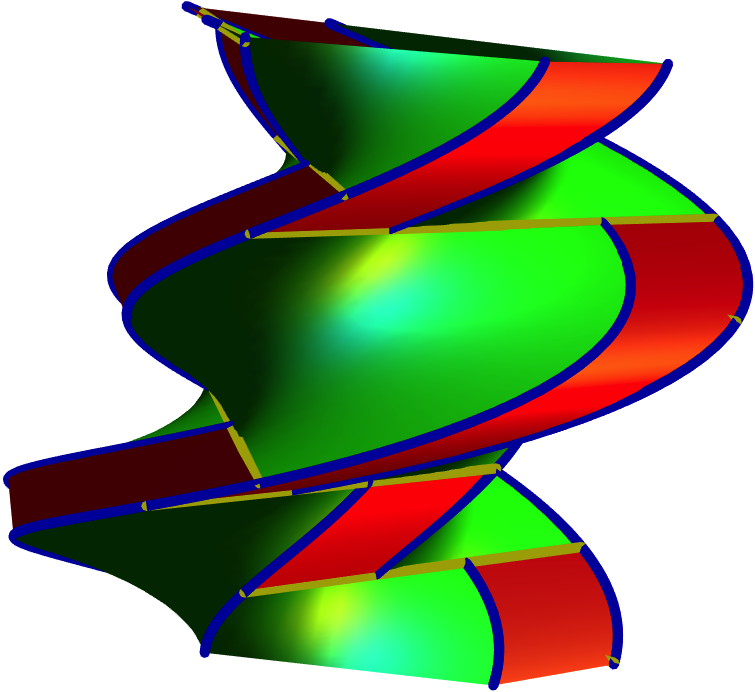
\includegraphics[width=0.95\columnwidth]{Figures/Title_picture}
            % }
          \end{center}
        }
      \end{minipage}
    \end{column}
  \end{columns}
\end{frame}


\section{Contact Surfaces Parameterization}
\begin{frame}
  \frametitle{Let it rotate\dots}
  We consider the rotation of the robot about a fixed point \(P \in \mathcal{W}\) such that  \(a\in\mathcal{A}\) is fixed to \(P\).
  \[P_a = \left\{ q \in \mathcal{C} \mid a(q) = P \right\}\]
  \vskip1ex
  \begin{minipage}{.4\linewidth}
    \begin{overlayarea}{\textwidth}{5cm}
      \begin{figure}
        \centering
        \begin{tikzpicture}
  \def\vRad{2pt}
  \tikzset{x=10pt,y=10pt}

  % Robot's vertices definition
  \coordinate (a1) at (6,0);
  \coordinate (a2) at (1,6);
  \coordinate (a3) at (-3.5,-1.0);
  \coordinate (a4) at (0,-3);
  \node[green,right=0.5em] at (a1){$a_1$};
  \node[green,right=0.5em] (ve) at (a2){$a_2$};
  \node[green,left=0.5em] at (a3){$a_3$};
  \node[green,below=0.5em] at (a4){$a_4$};

  % Robot's polygon
  \draw[line join=round,green,fill=green!20,line width=\vRad] (a1) -- (a2) -- (a3) -- (a4) -- (a1) -- cycle;
  \node[red] (R0) at (barycentric cs:a1=0.25,a2=0.25 ,a3=0.25,a4=0.25){};

  \only<1>{ 
    \fill[red] (R0) circle (\vRad) node[right=+0.5em] {$R_0=a$};
    \draw[->] ($(R0)+(30:1)$) arc (20:310:1);
  }

\only<2->{
  \fill[red!20] (R0) circle (\vRad) node[right=+0.5em] {$R_0$};
  \node[red] (a) at (barycentric cs:a1=0.3,a2=0.8 ,a3=0.3){};
  \fill[red] (a) circle (\vRad) node[right=+0.5em] {$a$};
%  \draw[->] ($(a)+(40:1)$) arc (40:240:1);
  \draw[->] (a) let \p1 = ($(R0)-(a)$) in  ++ (210: {veclen(\x1,\y1)}) arc (210:335:({veclen(\x1,\y1)});
  \draw[blue,<->] (a) -- node[right]{$r_a$} (R0);
}
  
  
  % Robot's vertices plotting
  \foreach \pts in {a1,a2,a3,a4}
  \fill [green!70] (\pts) circle (2*\vRad);  
  
\end{tikzpicture}

      \end{figure}
    \end{overlayarea}
  \end{minipage}
  \hfill
  \begin{minipage}{.4\linewidth}
    \begin{overlayarea}{\textwidth}{5cm}
      \only<1>{
        \vfill
        If \(a = R_0\) then \(P_a\) is a vertical \emph{straight} line.
      }
      \only<2->{
        \vfill
        If \(a\) is some arbitrary point in \(\mathcal{A}\) then \(P_a\) is a \emph{helix} with axis in the
        \(\theta\) direction.
        \vskip1ex
        \begin{tikzpicture}
          \begin{axis}[
            width=1.\linewidth,view={60}{30},xlabel=$x$,ylabel=$y$,zlabel=$\theta$,xtick={-1,0,1}, ytick={-0.5,0,1} ]
            \addplot3[red,domain=0:2*pi,samples=55,samples y=0] (
            {sin(deg(-x))}, {cos(deg(-x))}, {x} );
          \end{axis}
        \end{tikzpicture}
      }
  \end{overlayarea}
  \end{minipage}
\begin{overlayarea}{\textwidth}{1cm}
  \only<3->{
    \begin{block}{Remark}
      Helices cover \(\mathcal{C}\).
    \end{block}
  }
\end{overlayarea}
\end{frame}


\begin{frame}
  \frametitle{Parameterization of a Rotation}
  \begin{block}{Input}
    \begin{itemize}
    \item A robot \(\mathcal{A}\) and a point \(a\in\mathcal{A}\).
    \item A fixed point \(P \in \mathcal{W}\) in the work space.
    \end{itemize}
  \end{block}

  \begin{minipage}{0.45\linewidth}
    \begin{block}{The parameterization}
      \[
      q^P_a(\phi) = \binom{\vec{r}(\phi)}{\theta(\phi)} \in
      \mathcal{C}
      \]
      where:

    \begin{align*}
      \vec{r}(\phi) & =  P- R^{\phi} a\\
      \theta(\phi) & = \phi \mod 2\pi
    \end{align*}
  \end{block}
\end{minipage}
\hfill
\begin{minipage}{0.45\linewidth}
  \begin{block}{Added Value}
    Currently, if the robot and the obstacles are convex then \emph{exact
    bounds} of the free part of the contact surface can be found.
  \end{block}
\end{minipage}
\end{frame}

\begin{frame}
  \frametitle{Vertex-Edge Contact}
  \begin{columns}[c]
    \begin{column}{0.5\textwidth}
      \begin{minipage}[c][\textheight]{\columnwidth}
        \begin{itemize}
        \item<1-> Take the parameterization of rotation \(q^P_a(\phi) = \binom{P-R^{\phi} a}{\phi \mod 2\pi}\)
        \item<2-> Set \(P(t) = (1-t) b_j + t b_{j+1} \in E^{\mathcal{O}}_j\)
        \item<3-> Then%
          \[S(t,\phi)  = q ^{P(t)}_{a_i}(\phi)\]%
          is a \emph{developable surface} which parameterizes a \emph{vertex-edge} contact surface.
        \end{itemize}
      \end{minipage}
  \end{column}
  \begin{column}{0.45\textwidth}
    \begin{minipage}[c][\textheight]{\columnwidth}
      \centering
      \onslide<3>{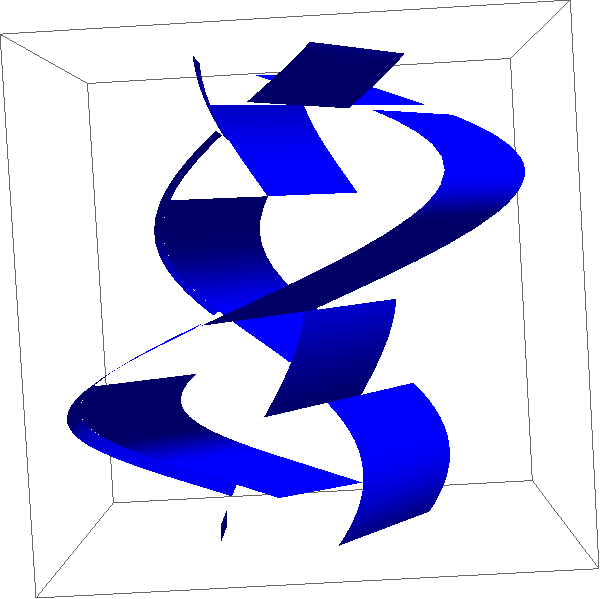
\includegraphics[width=0.9\columnwidth]{Figures/vecc}}
    \end{minipage}
  \end{column}
\end{columns}
\note<3->{Say that the surfaces have to become \textbf{patches}!}
\end{frame}

\begin{frame}
  \frametitle{Edge-Vertex Contact}
  \begin{columns}[c]
    \begin{column}{0.5\textwidth}
      \begin{minipage}[c][\textheight]{\columnwidth}
        \begin{itemize}
        \item<1-> Take the parameterization of rotation \(q^P_a(\phi) = \binom{P-R^{\phi} a}{\phi \mod 2\pi}\)
        \item<2-> Set \(a(t) = (1-t) a_i + t a_{i+1}\)
        \item<3-> Then \[S(t,\phi)  = q ^{b_j}_{a(t)}(\phi)\] is a \emph{non cylindrical ruled surface} which parameterizes an \emph{edge-vertex} contact surface.
        \end{itemize}
      \end{minipage}
    \end{column}
    \begin{column}{0.45\textwidth}
      \begin{minipage}[c][\textheight]{\columnwidth}
        \centering
        \onslide<3>{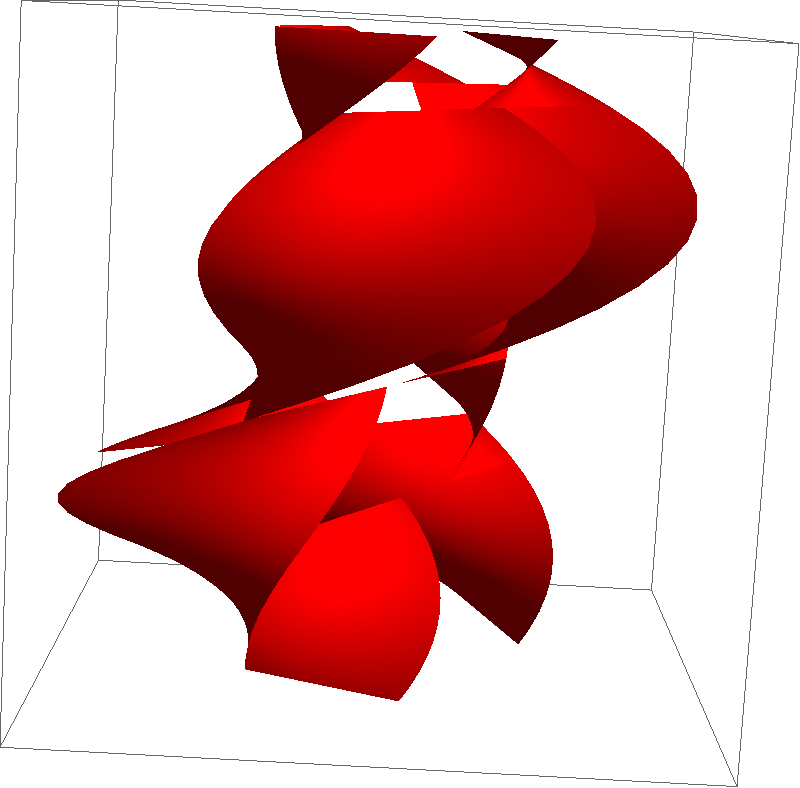
\includegraphics[width=0.9\columnwidth]{Figures/evcc}}
      \end{minipage}
    \end{column}
  \end{columns}
\end{frame}

\begin{frame}
  \frametitle{The Full Picture}
  \begin{minipage}[c][\textheight]{0.5\linewidth}
    \begin{itemize}
    \item<1-> For all possible vertex-edge and edge-vertex combinations we obtain the object to
      the right.
    \item<1-> In the convex case, we can easily compute the exact
      contact patches.
    \end{itemize}
  \end{minipage}
  \hfill
  \begin{minipage}[c][\textheight]{0.45\linewidth}
    \begin{figure}
      \centering
      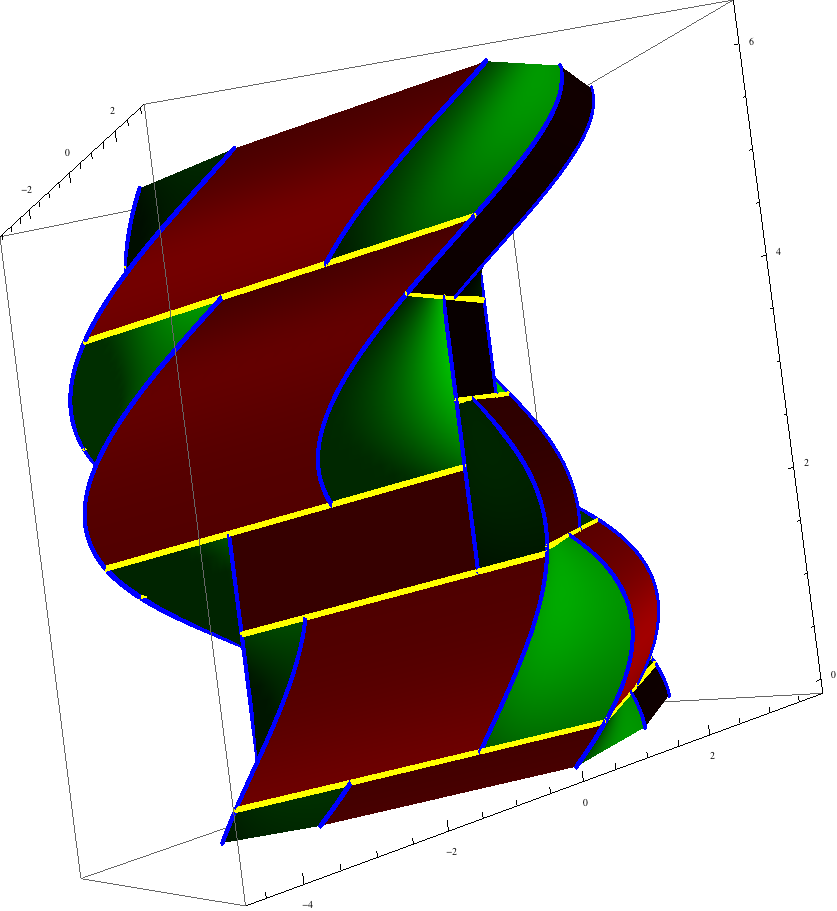
\includegraphics[width=0.95\linewidth]{Figures/full_contact}
    \end{figure}
  \end{minipage}
\end{frame}

\begin{frame}
  \frametitle{Be Rational!}
  \begin{block}{Drawback}
    In the introduced parameterization, non algebraic computations are
    needed. Thus, its accuracy in practical applications is limited.
  \end{block}
  \begin{block}{Rational Workaround}
    Set \(\psi=\tan \frac{\phi}{2}\) and %
    \(
    M^\psi = \frac{1}{1+\psi^2}\begin{pmatrix}
      1-\psi^2 & -2 \psi \\
      2\psi & 1-\psi^2
    \end{pmatrix}
    \) %
    we obtain a \emph{rational parameterization}
    \[
    k^P_a(\psi) = \left( \vec{r}(\psi),\tau(\psi)\right)
    \]
    where
    \begin{align*}
      \vec{r}(\psi) = & P - M^\psi a\\
      \tau(\psi) = & \psi
    \end{align*}
for \(\psi\in (-\infty,+\infty)\).
  \end{block}
\end{frame}

\section{Geometrical Properties}

\begin{frame}
  \frametitle{Vertex-Edge Contact Surface}
  \begin{minipage}{0.63\linewidth}
    The contact surface consists of translated copies of \emph{congruent}
    helix, therefore it is:
    \begin{itemize}
    \item Cylindrical
    \item Developable
    \item Has vanishing \emph{Gaussian curvature}
    \item The \emph{mean curvature} is identically \(0\) if and only if \(a_i = \vec{0}\). In this case, the surface is a vertical plane.
    \end{itemize}
  \end{minipage}
  \hfill
  \begin{minipage}{0.35\linewidth}
    \begin{figure}
      \centering
      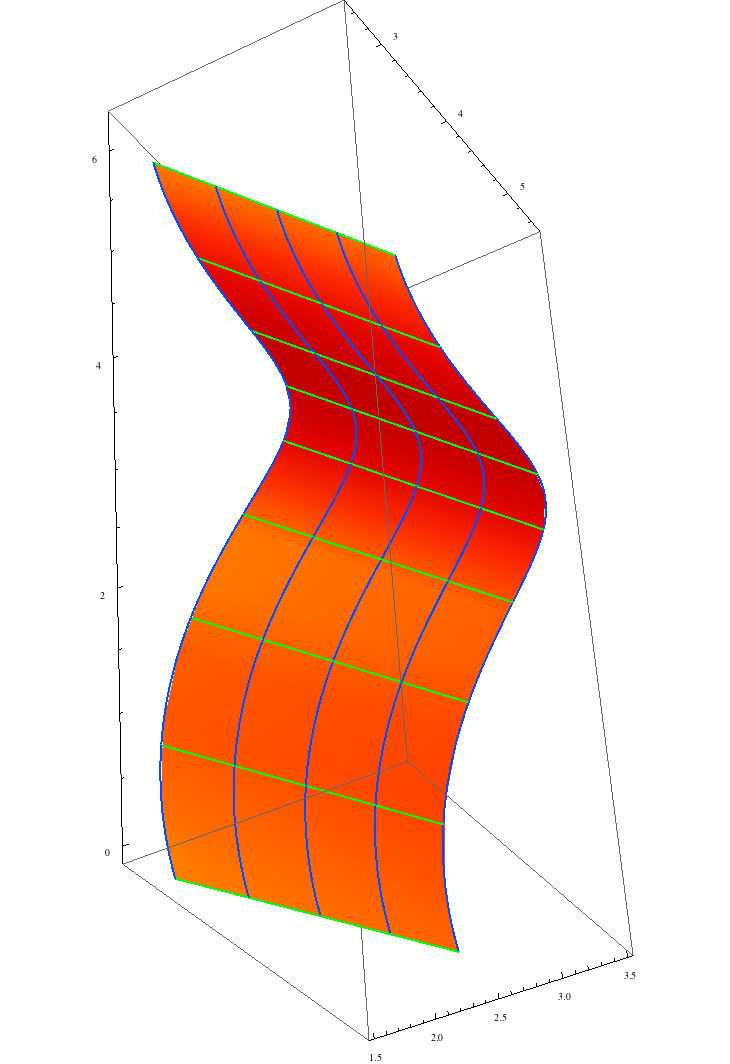
\includegraphics[height=0.9\textheight]{Figures/ve-full-contact}
    \end{figure}
  \end{minipage}
\end{frame}

\begin{frame}
  \frametitle{Edge-Vertex Contact Surface}
  \begin{minipage}{0.63\linewidth}
    \begin{itemize}
    \item Has negative \emph{Gaussian curvature}.
    \item The \emph{mean curvature} is identically \(0\) if the reference point
      is on the edge.
    \item Both curvatures depend \emph{only} on \(t\)
    \item The curvatures extrema are attained along the \emph{same}
      and \emph{unique} helix.
    \end{itemize}

    % \begin{center}
    %   \href{run:Demos/ev-curvatrue.app}{Demo Example}
    % \end{center}
  \end{minipage}
  \hfill
  \begin{minipage}{0.35\linewidth}
    \begin{figure}
      \centering
      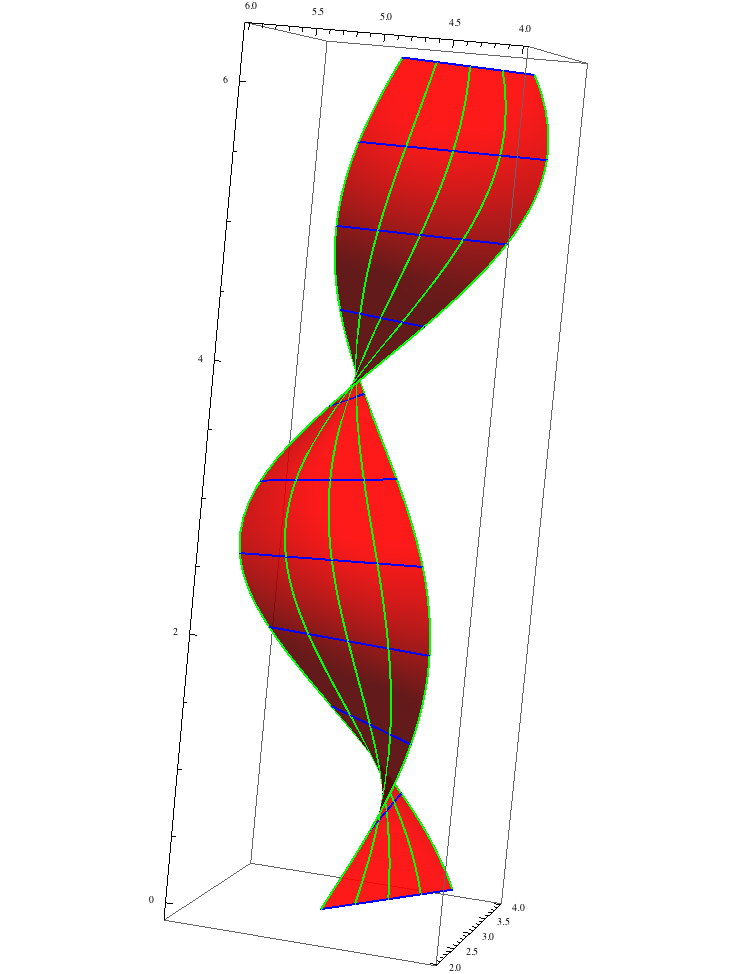
\includegraphics[height=0.95\textheight]{Figures/ev-full-contact}
    \end{figure}
  \end{minipage}
\end{frame}

\section{Summary}

\begin{frame}
  \frametitle{Recap}
  We considered:
  \begin{itemize}
  \item Parameterization of contact surfaces for polygonal robot in
    the plan.
  \item Geometrical analysis of the contact surfaces.
  \end{itemize}
  %
  % \vspace{5ex}
  %
  \onslide<2->{
    \begin{center}
      
\begin{tikzpicture}
        \node[rotate=-30,align=center] at (0,-2cm){%
          \begin{Huge}Thank you!\end{Huge}\\
          \texttt{dror.atariah@fu-berlin.de}
        };
      \end{tikzpicture}
    \end{center}

    \begin{center}
      \begin{tiny}
        \href{run:run_video}{Local video} / \href{http://www.youtube.com/watch?v=SBFwgR4K1Gk&feature=youtu.be&t=7m3s}{YouTube version}
      \end{tiny}
    \end{center}
  }
\end{frame}


% All of the following is optional and typically not needed.

\appendix
% \section<presentation>{References}
% \begin{frame}[allowframebreaks]{For Further Reading}
% \bibliographystyle{plain}
% \bibliography{/media/data/documents/BiBTeX/personalRef.bib}
% \end{frame}
\end{document}
